\section{CVaR model}\label{sec:CVaR}

The CVaR model was built based on the first set of scenarios with start date 2008-02-27, obtained from scenario generaion chapter. 
Based on this set the current value and expected value $P_{i,s}$ is determined for each ETF $i$ for each scenario $s$.
In addition, an initial budget of 1 million kr is considered.  
The CVaR model is defined as
\begin{align}
\sum_{i} x_{i} &= \up{Budget} \\
\up{MeanReturn} &\ge \mu_{\up{Target}} \up{Budget} \\
\up{VaRDev}_{s} &\ge \up{Losses}_{s} - \up{VaR} \; \; \forall s \\
\up{Losses}_{s} &= \sum_{i} x_{i} - \sum_{i} \up{P}_{i,s} x_{i} \; \; \forall s \\
\up{CVaR} &= \up{VaR} + \frac{1} {1 - \alpha} \sum_{s} \up{pr}_{s} \up{VaRDev}_{s} \\
\up{MeanReturn} &= \sum_{i} \up{EP}_{i} x_{i}
\end{align}
where $ \mu_{\up{Target}}$ is 0, $\up{P}_{i,s}$ is the value of each ETF $i$ by scenario $s$, $\up{pr}_{s}$ is the probability of each scenario $s$, $\up{EP}_{i}$ is the expected value for each ETF $i$, and $\alpha$ is assumed to be 0.5.
For this work, $\up{pr}_{s}$ is assumed to be linearly distributed over the scenarios, i.e. $\up{pr}_{s} = \frac{1}{|\Omega|} \forall s$.

\begin{figure}[tp]
\centering
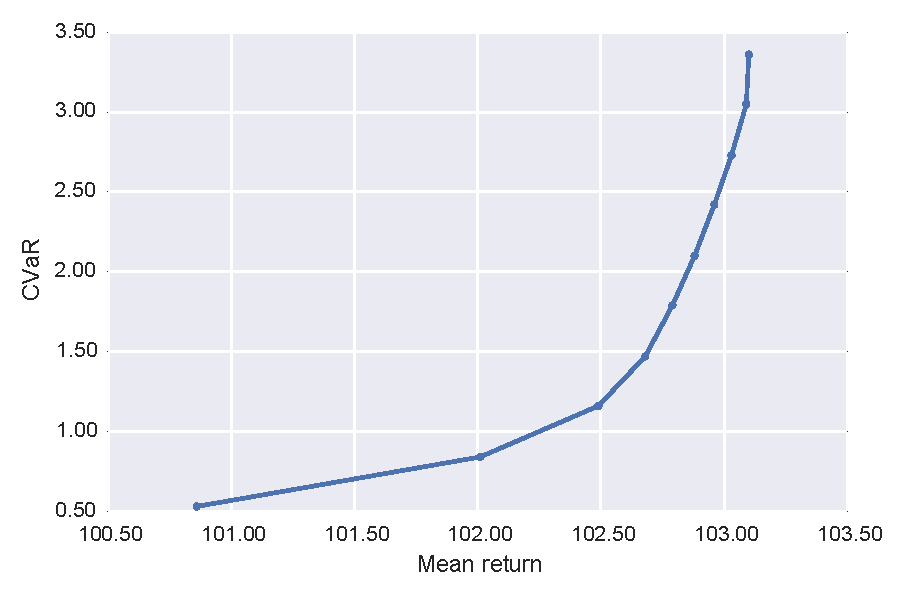
\includegraphics{../pic/frontier.pdf}
\caption{Optimal frontier for equidistant steps in CVaR. `Expected value' is the mean value of the portfolios found based on the scenarios.}
\label{fig:frontier}
\end{figure}

In order to obtain the efficient frontier based on 10 optimal solutions of CVaR model is neccesary to find the minimum CVaR solution, $\up{CVaR}_{\min}$, as well as $\up{CVaR}_{\max}$ from the maximization of mean return.
Between these extreme points, 10 values of $\up{CVaR}_{\up{Target}}$ are created by linear interpolation. 
A constraint for limit the space solution movement to the $\up{CVaR}_{\up{Target}}$ is included in the CVaR model, and is defined as
\begin{align}
\up{CVaR} &\le \up{CVaR}_{\up{Target}} 
\end{align}
For each of the 10 values, the CVaR model is optimized in order to maximize the MeanReturn variable. 
The efficient frontier of the 10 optimal solutions is presented in Figure~\ref{fig:frontier}.
At low CVaR, a small increase in CVaR leads to a large increase in expected return, whereas the opposite holds true for the high values of CVaR.


\begin{figure}[tp]
\centering
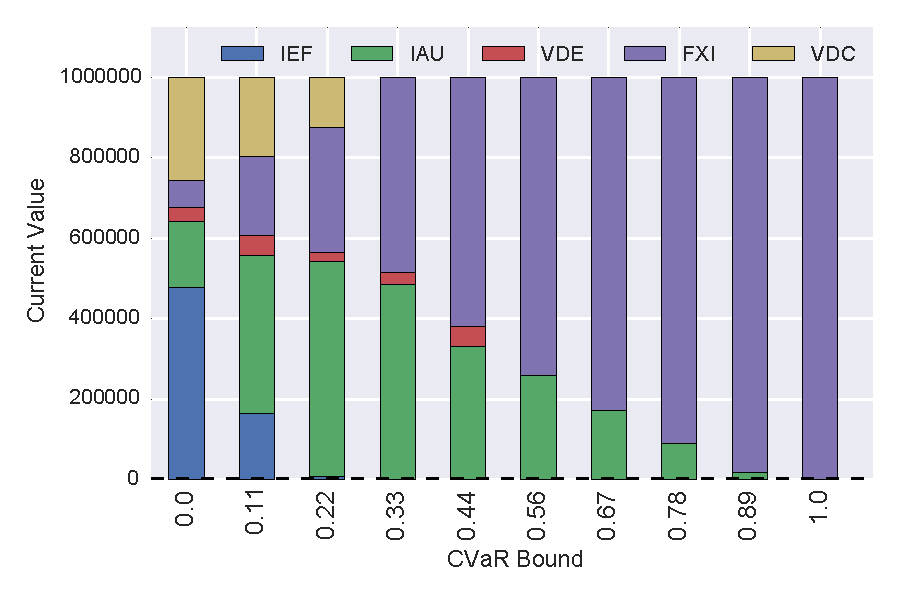
\includegraphics{../pic/Stake_vs_CVaR.pdf}
\caption{Portfolios at varying levels of the CVaR bound.}
\label{fig:scenarioportfolios}
\end{figure}

The portfolio results for each of the 10 runs is illustrated in Figure~\ref{fig:scenarioportfolios}.
A CVaR bound of 0.0 indicates that CVaR is minimal, with 1.0 indicating that the optimization solely considers mean return.
One can see that FXI index increases its weight in the portfolio according to the increase of CVaR target. 
This happens because the increase of CVaR target leads to the maximization of return.
In the period before the trading date (2008-02-27), the scenario generation contains the historical information for the last three years, where FXI index has a higher return when compared to other assets (as one can see in Figure~\ref{fig:prices_selected}).

\begin{figure}[tp]
\centering
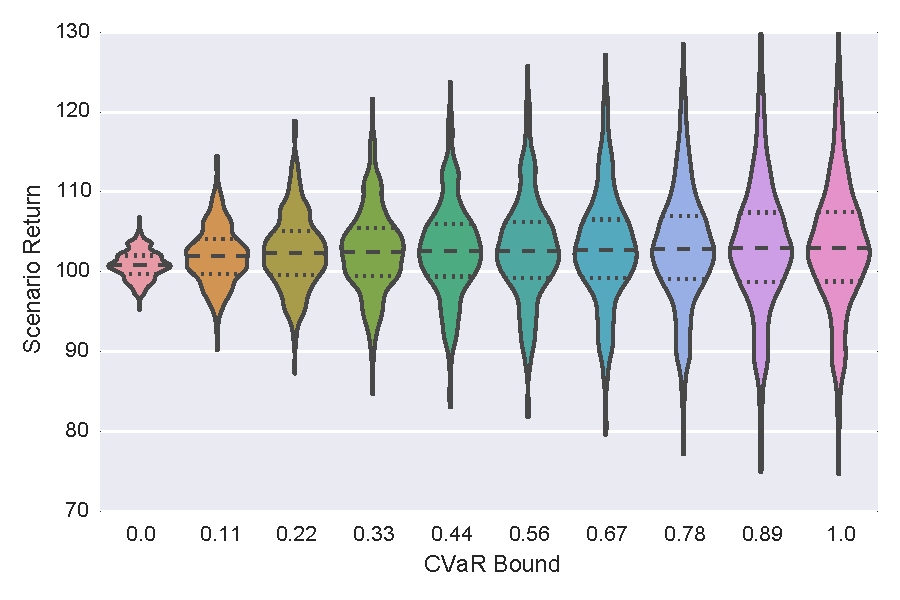
\includegraphics{../pic/Scenario_Return.pdf}
\caption{Scenario return for portfolios at varying levels of the CVaR bound.
The distributions for each bound are mirrored on the vertical axis, with the mean (dashed) and standard deviation (dotted) shown.}
\label{fig:scenarioreturn}
\end{figure}

Figure~\ref{fig:scenarioreturn} compares the scenario return at varying levels of the CVaR bound.
One can verify that the possibility of gettting higher return increase according to the increase of CVaR target  as expected.
It is also clear that we accept a very large increase in risk (corresponding to scenarios for which we lose money), in exchange for a relatively modest increase in expected return.


